% 原书 p.82–p.85（PDF p.90–p.93）
\section{可序性（Orderability）}

\begin{keytakeaways}
\begin{itemize}
  \item 几何图像：切触哈密顿动力学的独特现象是「平移常数」——把 $h_t$ 平移
        常数 $s$ 会额外扭上 Reeb 流 $\varphi_{R_\alpha}^{st}$（见 (3.42)），
        而在辛几何中常数函数不产生任何动力学差别。
  \item 数学工具：$\Op{Cont}_0(M,\xi)$ 的万有覆叠
        $\widetilde{\Op{Cont}_0}(M,\xi)$、非负/正同痕、偏序关系 (3.45)，
        以及判定准则（命题 3.7.1）。
  \item 本节结论：$(M,\xi)$ 可序当且仅当 $\Op{Cont}_0(M,\xi)$ 中不存在正的可缩
        环路；标准切触球面非可序，单位余球面丛与奇数维实射影空间可序。
\end{itemize}
\end{keytakeaways}

% >>> p090
到目前为止我们已经看到，切触哈密顿动力学与（辛的）哈密顿动力学最具标志性的
差别之一，是「平移常数」（见例 3.5.3）。确切地说，给定切触流形
$(M,\xi=\ker\alpha)$ 上同痕 $\{\varphi_t\}$（在 $\Op{Cont}_0(M,\xi)$ 中）
的切触哈密顿函数 $h:[0,1]\times M\to\R$，考虑把 $h$ 平移一个常数
$s\in\R$，形式为 $s+h_t\circ\varphi_{R_\alpha}^{-st}$。由习题 3.5.1，它生成
如下复合：
\begin{equation}\tag{3.42}
  \psi(s)_t:=\varphi_{R_\alpha}^{st}\circ\varphi_t,
  \qquad t\in[0,1].
\end{equation}
换言之，平移常数导致一次沿 Reeb 流的「扭转」（而在辛几何中，平移常数就
哈密顿动力学而言不产生任何差别）。

注意，对两个满足 $s\le s'$ 的实数，若 $s'-s$ 足够大（例如不小于
$\max_{t\in[0,1]}(\max_M h_t-\min_M h_t)$），就可以在切触哈密顿函数的层面上
比较、或者更确切地排序同痕 $\{\psi(s)_t\}$ 与 $\{\psi(s')_t\}$，即
\begin{equation}\tag{3.43}
  \{\psi(s)_t\}\preceq\{\psi(s')_t\}
  \ \Longleftrightarrow\
  s+h_t\circ\varphi_{R_\alpha}^{-st}
  \le s'+h_t\circ\varphi_{R_\alpha}^{-s't}
\end{equation}
对任意 $t\in[0,1]$ 在 $M$ 上逐点成立。这为 Eliashberg 与 Polterovich 在
[77] 中提出的\textbf{可序性}（orderability）提供了动机，它是切触几何中特有
的现象。

为了严格定义可序性，先回忆 $\Op{Cont}_0(M,\xi)$ 的万有覆叠，记为
$\widetilde{\Op{Cont}_0}(M,\xi)$。它由 $\Op{Cont}_0(M,\xi)$ 中的同痕
（如图 3.14 所示）模去同伦关系构成。确切地说，
\[
  \widetilde{\Op{Cont}_0}(M,\xi)
  :=\bigl\{[\{\varphi_t\}]\ \big|\ \varphi_0=\mathbf{1},\ t\in[0,1]\bigr\},
\]
其中 $\{\varphi_t\}$ 与 $\{\psi_t\}$ 等价，当且仅当它们在固定端点下光滑同伦
（见图 3.15）。注意单位元 $[\mathbf{1}]
\in\widetilde{\Op{Cont}_0}(M,\xi)$ 表示 $\Op{Cont}_0(M,\xi)$ 中可缩环路
（端点回到 $\mathbf{1}$）的类。容易验证
$\widetilde{\Op{Cont}_0}(M,\xi)$ 是群，单位元为 $[\mathbf{1}]$，乘法由
$[\{\varphi_t\}]\cdot[\{\psi_t\}]:=[\{\varphi_t\circ\psi_t\}]$ 给出。

有一个自然的群同态
$\pi:\widetilde{\Op{Cont}_0}(M,\xi)\to\Op{Cont}_0(M,\xi)$，它由「钉住
时间 $1$ 的映射」定义：
\begin{equation}\tag{3.44}
  \pi\bigl([\{\varphi_t\}]\bigr):=\varphi_1
\end{equation}
对任意类 $[\{\varphi_t\}]\in\widetilde{\Op{Cont}_0}(M,\xi)$ 成立。一个有趣
的观察是 $\ker\pi=\pi_1(\Op{Cont}_0(M,\xi))$。这意味着，从 §3.5 中切触
哈密顿动力学的视角看，在 $\widetilde{\Op{Cont}_0}(M,\xi)$（而不是
$\Op{Cont}_0(M,\xi)$）上工作有时会产生歧义：因为
$\pi_1(\Op{Cont}_0(M,\xi))$ 会起作用，可能扰动切触哈密顿函数的选取（后者
等价于类 $[\{\varphi_t\}]$ 中代表元的选取）。

% >>> p091
\begin{figure}[htbp]
  \centering
  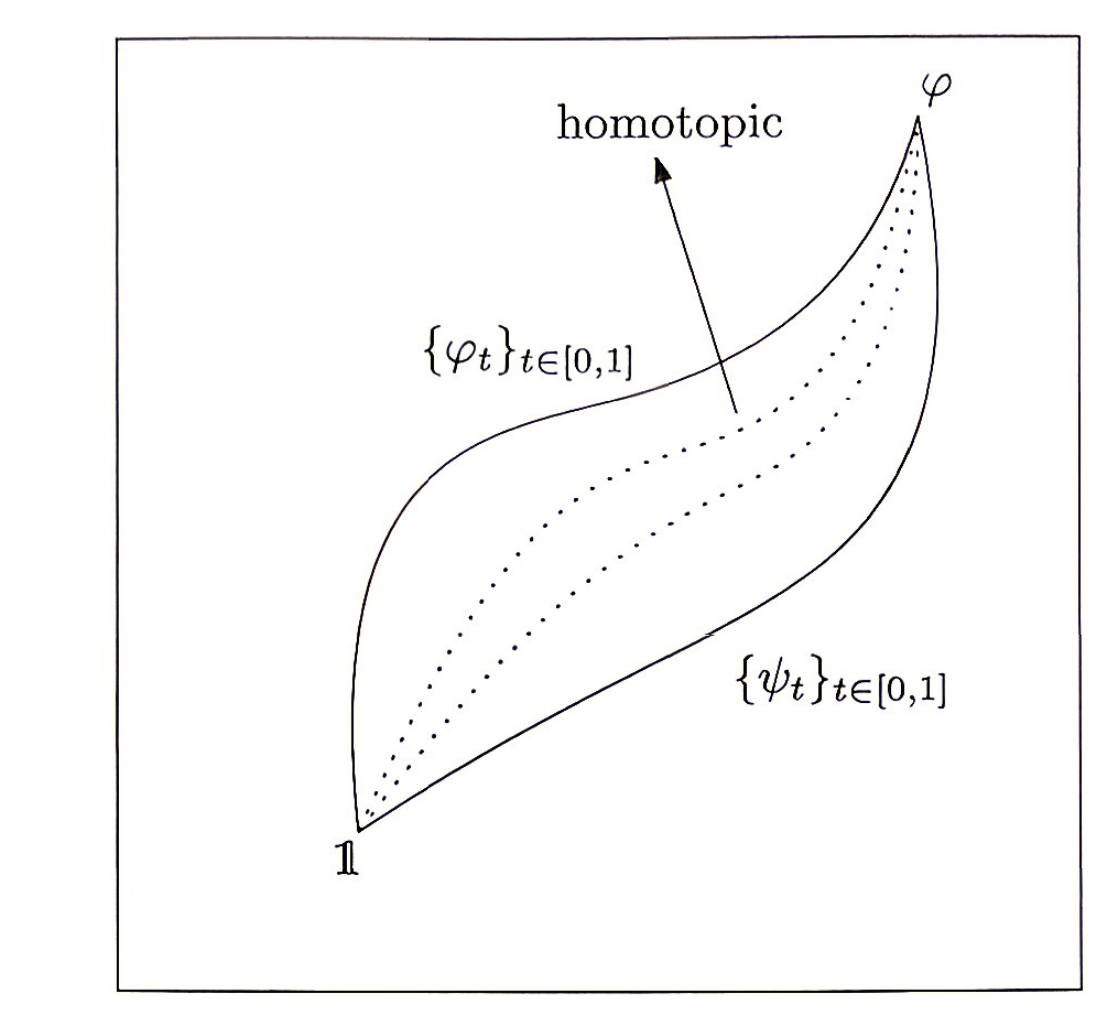
\includegraphics[width=0.42\linewidth]{figures/fig_p091_1.png}
  \caption*{图 3.15\quad $\Op{Cont}_0(M,\xi)$ 中的一条道路同伦
  （原书 p.83, Figure 3.15）}
\end{figure}

\begin{wdefn}{3.7.1}
设 $(M,\xi)$ 是切触流形。称 $\Op{Cont}_0(M,\xi)$ 中的同痕 $\{\varphi_t\}$
是\textbf{非负的}（相应地，\textbf{非正的}），若对 $(M,\xi)$ 的
\textbf{任意}切触 $1$-形式 $\alpha$，由命题 3.5.1 给出的切触哈密顿函数
$h:[0,1]\times M\to\R$ 对任意 $t\in[0,1]$ 都是 $M$ 上逐点非负（相应地，
非正）的函数。若 $h_t$ 对任意 $t\in[0,1]$ 都逐点为正（相应地，为负），则
称 $\{\varphi_t\}$ 为\textbf{正的}（相应地，\textbf{负的}）同痕。
\end{wdefn}

% [Tutor Note: 原文疑误——定义 3.7.1 开头写作「设 $(M,\omega)$ 是切触流形」，
% 其中 $\omega$ 应为 $\xi$：本定义的通篇都只用切触结构 $\xi$ 与切触
% $1$-形式 $\alpha$，$(M,\omega)$ 的写法是从辛几何部分沿用而来的笔误。已记入
% review_ch03.md。]

\begin{wrem}{3.7.1}
同痕 $\{\varphi_t\}$ 是否非负或为正，实际上与切触 $1$-形式的选择无关，因为
（同一 $\xi$ 的）两个不同切触 $1$-形式相差 $M$ 上的一个正函数。
\end{wrem}

% [Tutor Note: 易错预警——注意定义 3.7.1 量词是「\textbf{任意}切触
% $1$-形式 $\alpha$」：若 $\alpha$ 换成 $\ee^f\alpha$，则切触哈密顿函数变为
% $\ee^f h_t$（见 (3.30) 第一式），正性仍保持；故「对某个 $\alpha$ 非负」与
% 「对任意 $\alpha$ 非负」等价（正函数因子不改变符号）。这条等价正是注 3.7.1
% 的内容，也是命题 3.7.1 与定义 3.7.2 不依赖 $\alpha$ 的原因。]

\begin{wexam}{3.7.1}
对 (3.42) 中的同痕，当 $M$ 紧时，只要 $s$ 足够大它就是正的。换言之，经
(3.42) 中的 Reeb 流扭转之后，$\Op{Cont}_0(M,\xi)$ 中任何同痕都可以成为
正同痕（只要 $M$ 紧）。\hfill$//$
\end{wexam}

(3.43) 中的排序可作如下解释：当 $s'-s$ 足够正时，下述复合
\[
  \bigl\{\psi(s)_t^{-1}\circ\psi(s')_t\bigr\}
\]
是非负同痕。这本质上归因于习题 3.5.1 的第二个结论，因为该同痕的切触
哈密顿函数（在相差一个正函数的意义下）正比于
\begin{align*}
  &\bigl(s'+h_t\circ\varphi_{R_\alpha}^{-s't}\bigr)
  -\bigl(s+h_t\circ\varphi_{R_\alpha}^{-st}\bigr)\\
  &\qquad=(s'-s)
  -\bigl(h_t\circ\varphi_{R_\alpha}^{-st}
  -h_t\circ\varphi_{R_\alpha}^{-s't}\bigr)\ge0,
\end{align*}
按我们的假设，它对任意 $t\in[0,1]$ 在 $M$ 上逐点成立。

为简洁起见，我们用 $\varphi$ 或 $\psi$ 表示
$\widetilde{\Op{Cont}_0}(M,\xi)$ 中的类。考虑下述推广 (3.43) 的关系：
\begin{equation}\tag{3.45}
  \varphi\preceq\psi
  \ \Longleftrightarrow\
  \varphi^{-1}\circ\psi\ \text{有非负代表元}.
\end{equation}
% >>> p092
例如，若 $\varphi$ 有非负代表元，则 $[\mathbf{1}]\preceq\varphi$。一个
直接的问题是：$\preceq$ 是否在
$\widetilde{\Op{Cont}_0}(M,\xi)$ 上定义偏序？确切地说，下述三条公理是否
成立：
\begin{enumerate}[label=(\roman*)]
  \item 对任意 $\varphi$，有 $\varphi\preceq\varphi$。
  \item 若 $\varphi\preceq\psi$ 且 $\psi\preceq\varphi$，则 $\varphi=\psi$。
  \item 若 $\varphi\preceq\psi$ 且 $\psi\preceq\theta$，则
        $\varphi\preceq\theta$。
\end{enumerate}
显然公理 (i) 与 (iii) 成立，非平凡的部分在公理 (ii)。有趣的是，公理 (ii)
未必总成立。我们仔细看一个例子。

\begin{wexam}{3.7.2}
例如，考虑一个正同痕 $\{\varphi_t\}$，使得 $[\{\varphi_t\}]=[\mathbf{1}]$，
即 $\{\varphi_t\}$ 是 $\Op{Cont}_0(M,\xi)$ 中的正的可缩环路。不失一般性，
设在 $t=1/2$ 处 $\varphi_{1/2}\neq\mathbf{1}$。则考虑下述两条同痕（都从
$\mathbf{1}$ 出发、终止于 $\varphi_{1/2}$）：
\[
  \{\varphi_t\}_{t\in[0,1/2]}
  \quad\text{与}\quad
  \{\psi_t:=\varphi_{1-t}\}_{t\in[0,1/2]}.
\]
第一条同痕是正的，而第二条同痕是负的。同时它们同伦（因为
$\{\varphi_t\}_{t\in[0,1]}$ 可缩）。因此，在
$\widetilde{\Op{Cont}_0}(M,\xi)$ 中
$[\{\varphi_t\}]=[\{\psi_t\}]$（见图 3.16）。综上可得
$[\{\varphi_t\}]=[\{\psi_t\}]\preceq[\mathbf{1}]
\preceq[\{\varphi_t\}]$，但 $[\{\varphi_t\}]\neq[\mathbf{1}]$，因为它们在
(3.44) 的映射 $\pi$ 下像不同。\hfill$//$
\end{wexam}

\begin{figure}[htbp]
  \centering
  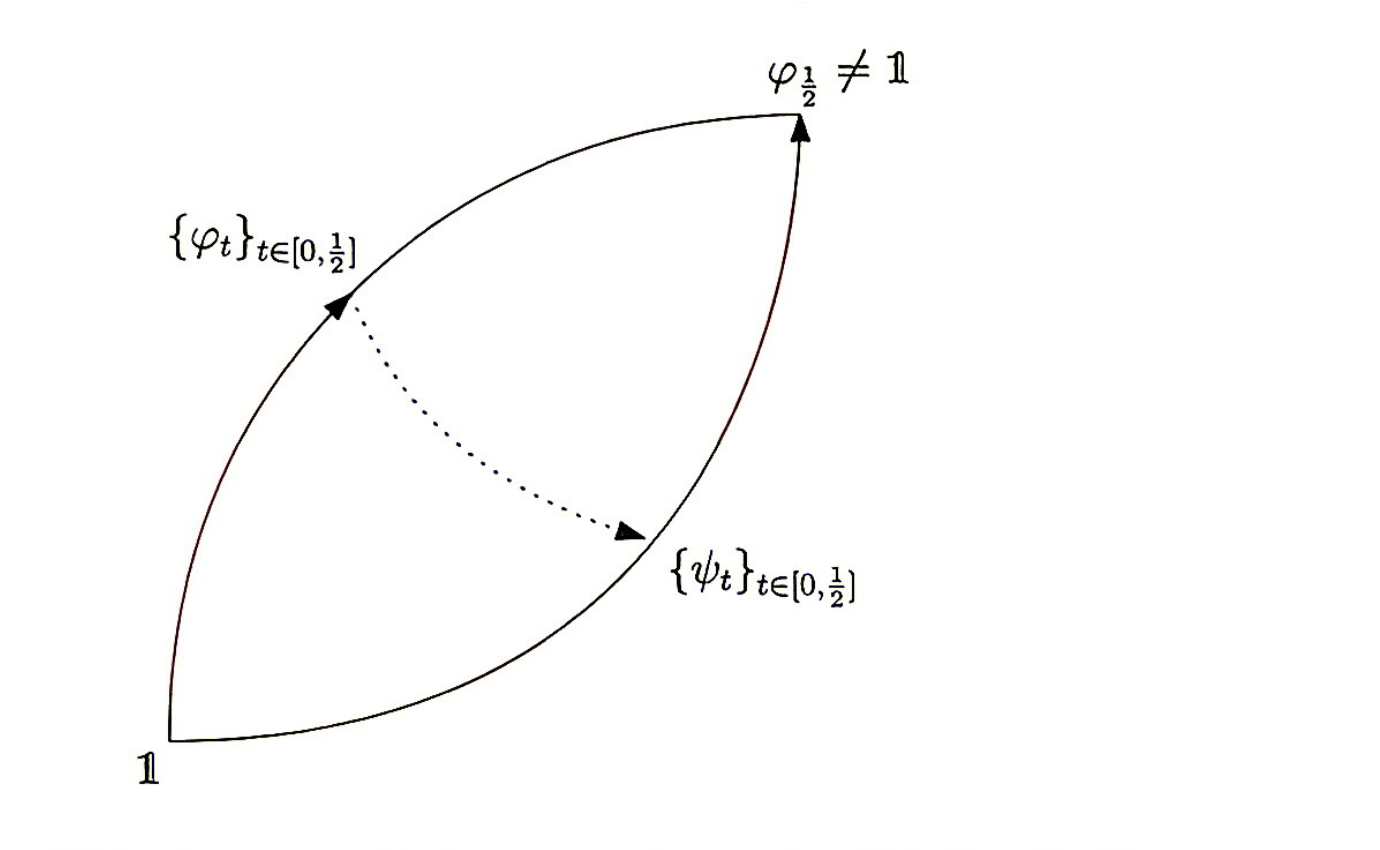
\includegraphics[width=0.52\linewidth]{figures/fig_p092_1.png}
  \caption*{图 3.16\quad 群 $G$ 中一条非常值的非负可缩环路
  （原书 p.84, Figure 3.16）}
\end{figure}

上面的例 3.7.2 表明：群 $\widetilde{\Op{Cont}_0}(M,\xi)$ 中存在正的可缩
环路，是 $\preceq$ 在 $\widetilde{\Op{Cont}_0}(M,\xi)$ 上成为偏序的障碍。
事实上，下述命题断言这是唯一的障碍。

\begin{wprop}{3.7.1}（[77] 中准则 1.2.C）
关系 (3.45) 是 $\widetilde{\Op{Cont}_0}(M,\xi)$ 上的偏序，当且仅当
$\Op{Cont}_0(M,\xi)$ 中不存在任何正的可缩环路。
\end{wprop}

\begin{wproof}
例 3.7.2 证明了「仅当」方向。这里给出「当」方向的证明。如上所述，我们
只需验证公理 (ii)，因为其他公理平凡地成立。假设 $\preceq$ 不满足公理
(ii)，则存在 $\varphi,\psi\in\widetilde{\Op{Cont}_0}(M,\xi)$，使得
$\varphi\preceq\psi$、$\psi\preceq\varphi$，但 $\varphi\neq\psi$。经共轭
变换，不妨设 $\psi=[\mathbf{1}]$。于是由 (3.45) 知
\[
  \varphi\preceq[\mathbf{1}]
  \ \Longrightarrow\
  \text{存在非正的 }\{\varphi_t\}_{t\in[0,1]},\
  [\{\varphi_t\}]=\varphi .
\]
类似地，再由 (3.45) 知
\[
  [\mathbf{1}]\preceq\varphi
  \ \Longrightarrow\
  \text{存在非负的 }\{\psi_t\}_{t\in[0,1]},\
  [\{\psi_t\}]=\varphi .
\]
特别地，$\varphi_1=\psi_1$。现在考虑
\[
  \theta_t:=
  \begin{cases}
    \psi_{2t}, & t\in[0,1/2],\\
    \varphi_{2-2t}, & t\in[1/2,1].
  \end{cases}
\]
这定义了 $\Op{Cont}_0(M,\xi)$ 中的一条非负同痕，且容易验证
$\{\theta_t\}_{t\in[0,1]}$ 也是可缩的，因为
$[\{\varphi_t\}]=\varphi=[\{\psi_t\}]$ 蕴含 $\{\varphi_t\}$ 与
$\{\psi_t\}$ 同伦。这就完成了证明。
\end{wproof}

% [Tutor Note: 含糊点拨——证明中「经共轭变换，不妨设 $\psi=[\mathbf{1}]$」
% 用到 $\preceq$ 在左乘（或共轭）下的不变性：若 $\varphi\preceq\psi$，
% 则 $\theta^{-1}\varphi\preceq\theta^{-1}\psi$（因为
% $(\theta^{-1}\varphi)^{-1}(\theta^{-1}\psi)
% =\varphi^{-1}\psi$），故可把 $\psi$ 化为单位元。另注意
% $\{\theta_t\}$ 的「非负性」来自两段分别非负；在其拼接点
% $t=1/2$ 处，$M$ 上逐点的非负性不受影响。]

现在可以给出切触流形可序性的定义了。

\begin{wdefn}{3.7.2}（见 [76] 中 §1.4）
称切触流形 $(M,\xi)$ 是\textbf{可序的}（orderable），若关系 (3.45) 是
$\widetilde{\Op{Cont}_0}(M,\xi)$ 上的偏序；否则称 $(M,\xi)$ 为
\textbf{非可序的}（non-orderable）。
\end{wdefn}

\begin{wrem}{3.7.2}
结合注 3.7.1 并直接由命题 3.7.1 看出：切触流形 $(M,\xi)$ 是否可序，与
切触结构 $\xi$ 的切触 $1$-形式的选取无关。
\end{wrem}

自可序性被提出以来，对（非）可序切触流形进行分类就成为切触几何的核心问题
之一。这一问题通常要借助切触几何中一些硬工具来处理。下面给出若干结果。

% >>> p093
\begin{wexam}{3.7.3}（[76] 中定理 1.10，[173]）
设 $n\ge2$。标准切触球面 $(S^{2n-1},\xi_{\mathrm{std}})$ 是非可序的。\hfill$//$
\end{wexam}

\begin{wexam}{3.7.4}（[76] 中定理 1.18，[47] 中推论 9.1）
单位余球面丛 $(S^*_gM,\xi=\lambda_{\mathrm{can}}|_{S^*_gM})$ 是可序的。\hfill$//$
\end{wexam}

\begin{wexam}{3.7.5}（[95]）
设 $n\ge2$。则奇数维实射影空间
$(\RP^{2n-1},\xi_{\mathrm{std}})$ 是可序的。这里切触结构
$\xi_{\mathrm{std}}$ 是 $S^{2n-1}$ 上标准切触结构
$\xi_{\mathrm{std}}$ 的 $\Z_2$-商。\hfill$//$
\end{wexam}
